% Double Arrows a la Chef
% Author: Dominik Haumann
\documentclass{article}
\usepackage{tikz}
\usetikzlibrary{arrows, decorations.markings}

% for double arrows a la chef
% adapt line thickness and line width, if needed
\tikzstyle{vecArrow} = [thick, decoration={markings,mark=at position
   1 with {\arrow[semithick]{open triangle 60}}},
   double distance=1.4pt, shorten >= 5.5pt,
   preaction = {decorate},
   postaction = {draw,line width=1.4pt, white,shorten >= 4.5pt}]
\tikzstyle{innerWhite} = [semithick, white,line width=1.4pt, shorten >= 4.5pt]

\begin{document}

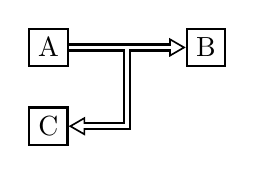
\begin{tikzpicture}[thick]
  \node[draw,rectangle] (a) {A};
  \node[inner sep=0,minimum size=0,right of=a] (k) {}; % invisible node
  \node[draw,rectangle,right of=k] (b) {B};
  \node[draw,rectangle,below of=a] (c) {C};

  % 1st pass: draw arrows
  \draw[vecArrow] (a) to (b);
  \draw[vecArrow] (k) |- (c);

  % 2nd pass: copy all from 1st pass, and replace vecArrow with innerWhite
  \draw[innerWhite] (a) to (b);
  \draw[innerWhite] (k) |- (c);

  % Note: If you have no branches, the 2nd pass is not needed
\end{tikzpicture}

\end{document}
